\documentclass[a4paper,12pt]{article}

\usepackage{graphicx}
\usepackage{wrapfig}
\usepackage{amsmath}
\usepackage{amsfonts}
\usepackage[english, russian]{babel}
\usepackage[T1, T2A]{fontenc}
\usepackage[utf8]{inputenc}
\usepackage{geometry}
\usepackage{indentfirst}
\usepackage{listings}
\usepackage[dvipsnames]{xcolor}
\usepackage[colorlinks]{hyperref}
\usepackage{amsmath}
\usepackage{float}
\usepackage{braket} 
\graphicspath{ {./images/} }
\geometry{left=2cm, right=2cm, bottom=2cm, top=2cm}

\hypersetup{
    linkcolor=blue,
    filecolor=magenta,
    urlcolor=cyan
}

\lstset{
    backgroundcolor=\color{white},
    basicstyle=\footnotesize\ttfamily,
    breaklines=true,
    frame=single,
    numbers=left,
    numberstyle=\tiny\color{gray},
    keywordstyle=\color{blue},
    commentstyle=\color{green!40!black},
    stringstyle=\color{darkblue},
    showstringspaces=false,
    tabsize=4,
    language=Mathematica
}

\definecolor{codegreen}{rgb}{0,0.6,0}
\definecolor{codegray}{rgb}{0.5,0.5,0.5}
\definecolor{codepurple}{rgb}{0.58,0,0.82}
\definecolor{backcolour}{rgb}{0.95,0.95,0.92}


\lstdefinestyle{codestyle}{
    backgroundcolor=\color{backcolour},
    commentstyle=\color{codegreen},
    keywordstyle=\color{blue},
    numberstyle=\tiny\color{codegray},
    stringstyle=\color{magenta},
    basicstyle=\ttfamily\footnotesize,
    breakatwhitespace=false,
    breaklines=true,
    captionpos=b,
    keepspaces=true,
    numbers=left,
    numbersep=5pt,
    showspaces=false,
    showstringspaces=false,
    showtabs=false,
    tabsize=2
}













\lstset{style=codestyle}
\lstset{extendedchars=\true}

\begin{document}
\begin{titlepage}
    \centering
    \vspace*{1cm}

    {\large Министерство науки и высшего образования Российской Федерации}\\
    {\large ФЕДЕРАЛЬНОЕ ГОСУДАРСТВЕННОЕ АВТОНОМНОЕ ОБРАЗОВАТЕЛЬНОЕ УЧРЕЖДЕНИЕ ВЫСШЕГО ОБРАЗОВАНИЯ «НАЦИОНАЛЬНЫЙ ИССЛЕДОВАТЕЛЬСКИЙ УНИВЕРСИТЕТ ИТМО»}\\
    {\large (УНИВЕРСИТЕТ ИТМО)}\\

    \vspace{2cm}

    {\large Факультет «Систем управления и робототехники»}\\

    \vspace{3cm}

    \textbf{{\Huge ОТЧЕТ}\\
    {\Huge О ЛАБОРАТОРНОЙ РАБОТЕ №3}}\\

    \vspace{1cm}

    {\LARGE По дисциплине «Частотные методы»}\\
    {\LARGE на тему: «Жесткая фильтрация»}\\

    \vspace{3cm}

    {\Large Студент:}\\
    Охрименко Ева

    \vspace{2cm}

    {\Large Преподаватели:}\\
    Догадин Егор Витальевич\\
    Пашенко Артем Витальевич\\

    \vspace{3cm}
    {\large г. Санкт-Петербург}\\
    {\large 2025}

\end{titlepage}
\newpage
\tableofcontents
\newpage

\section{Task. Жесткие фильтры}
\subsection{Краткое условие}

Рассмотрите функцию \( g(t) \), заданную как:
\[
g(t) = 
\begin{cases} 
a, & t \in [t_1, t_2], \\
0, & t \notin [t_1, t_2],
\end{cases}
\]
и её зашумлённую версию:
\[
u(t) = g(t) + b\xi(t) + c \sin(dt),
\]
где \(\xi(t) \sim U[-1, 1]\) — белый шум, а \( b, c, d \) — параметры.

\begin{itemize}
\item При \( c = 0 \) найдите Фурье-образ \( u(t) \), обнулите его вне \([- \nu_0, \nu_0]\) и выполните обратное преобразование. Исследуйте влияние \( \nu_0 \) и \( b \).

\item При ненулевых \( b, c, d \) обнулите Фурье-образ на выбранных частотах, подавляя шум и гармонику. Исследуйте влияние параметров.

\item бнулите Фурье-образ в окрестности \( \nu = 0 \), пропустите сигнал через фильтр и оцените результат.
\end{itemize}
\textbf{Ожидаемые результаты:} \\
Графики исходного, зашумлённого и фильтрованного сигналов, а также их Фурье-образов. Выводы по каждому пункту.

\subsection{Убираем высокие частоты}
\subsubsection{Предподготовка}
Для начала выберу все нужные параметры для этого задания:
\[
a = 4, t_0 = 0, t_1 = 3, c = 0, d = 5, b = 0.5
\]

Тогда у меня получится прямоугольная функция:\[
g(t) = 
\begin{cases} 
4, & t \in [0, 3], \\
0, & t \notin [0, 3],
\end{cases}
\]

Теперь посмотрим, какая функция белого шума получилась:
\[
u(t) = g(t) + 0.5\xi(t) + 0\sin(dt),
\]
где \(\xi(t) \sim U[-1, 1]\) — равномерное распределение на интервале \([-1, 1]\).

Слагаемое с синусом отсутствует, поэтому колебаний у шума также не будет. 

Теперь посмотрим на график функций \(g(t)\) и \(u(t)\):

\begin{figure}[H]  
    \centering
    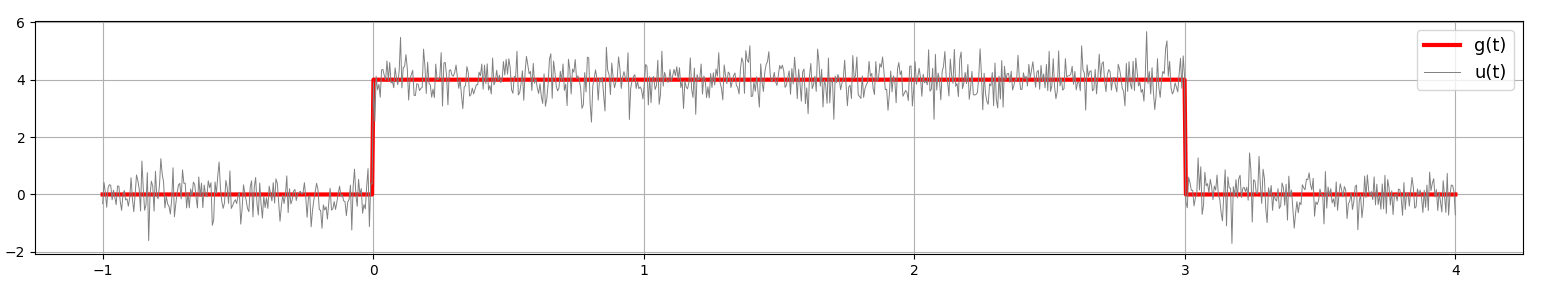
\includegraphics[width=1\textwidth]{../images/signalShum.png}
    \caption{График \(g(t)\) и \(u(t)\)}  
    \label{fig:my_image}  
\end{figure}
\hypertarget{mytext}{
Дальше в задании нужно найти фурье-образ \(u(t)\), обнулить его значение на диапазоне \([- \nu_0, \nu_0]\)
и восстановить сигнал с помощью обратного преобразования фурье.
}
\subsubsection{Фиксирую \(b\)}

Для начала выберем значения \(\nu_0 = 0.5\) и \(b = 0.5\). Теперь посмотрим на график
получившегося отфильтрованного сигнала при этих значениях. Также я приведу графики 
модулей фурье образов сигнала \(g(t)\), зашумленного сигнала \(u(t)\) и отфильтрованного сигнала.

\begin{figure}[H]  
    \centering
    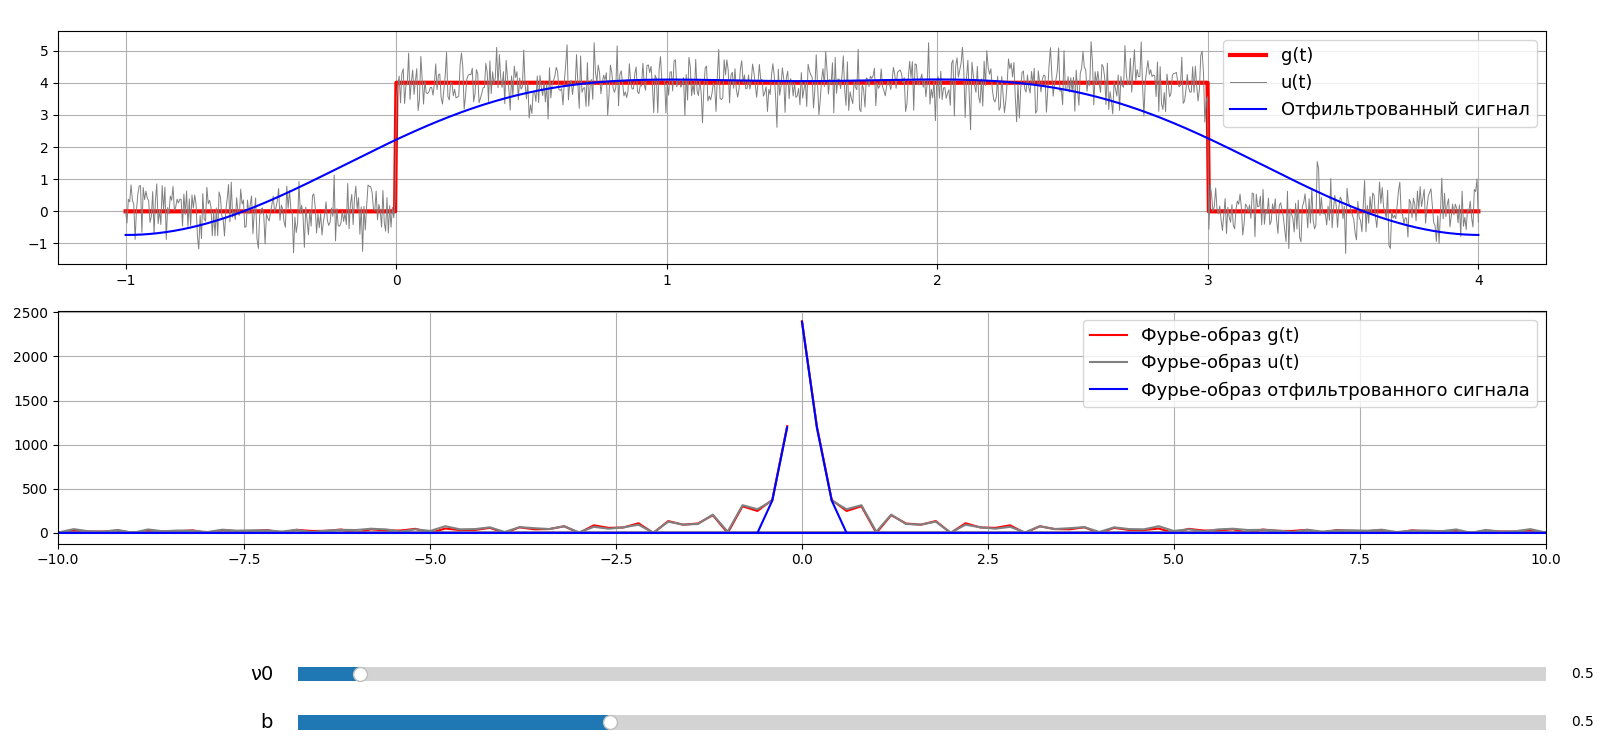
\includegraphics[width=1\textwidth]{../images/1.1_0.5_0.5.png}
    \caption{Графики при \(\nu_0 = 0.5\) и \(b = 0.5\)}  
    \label{fig:my_image}  
\end{figure}


Внизу можно заметить 2 бегунка, с помощью которых можно менять параметры.
В этой части задания я зафиксирую параметр \(b = 0.5\) и буду исследовать влияние
на поведение функций параметра \(\nu_0\). Выберу несколько \(\nu_0 = \set{1, 1.5, 3, 10}\)
и отрисую графики:

\begin{figure}[H]  
    \centering
    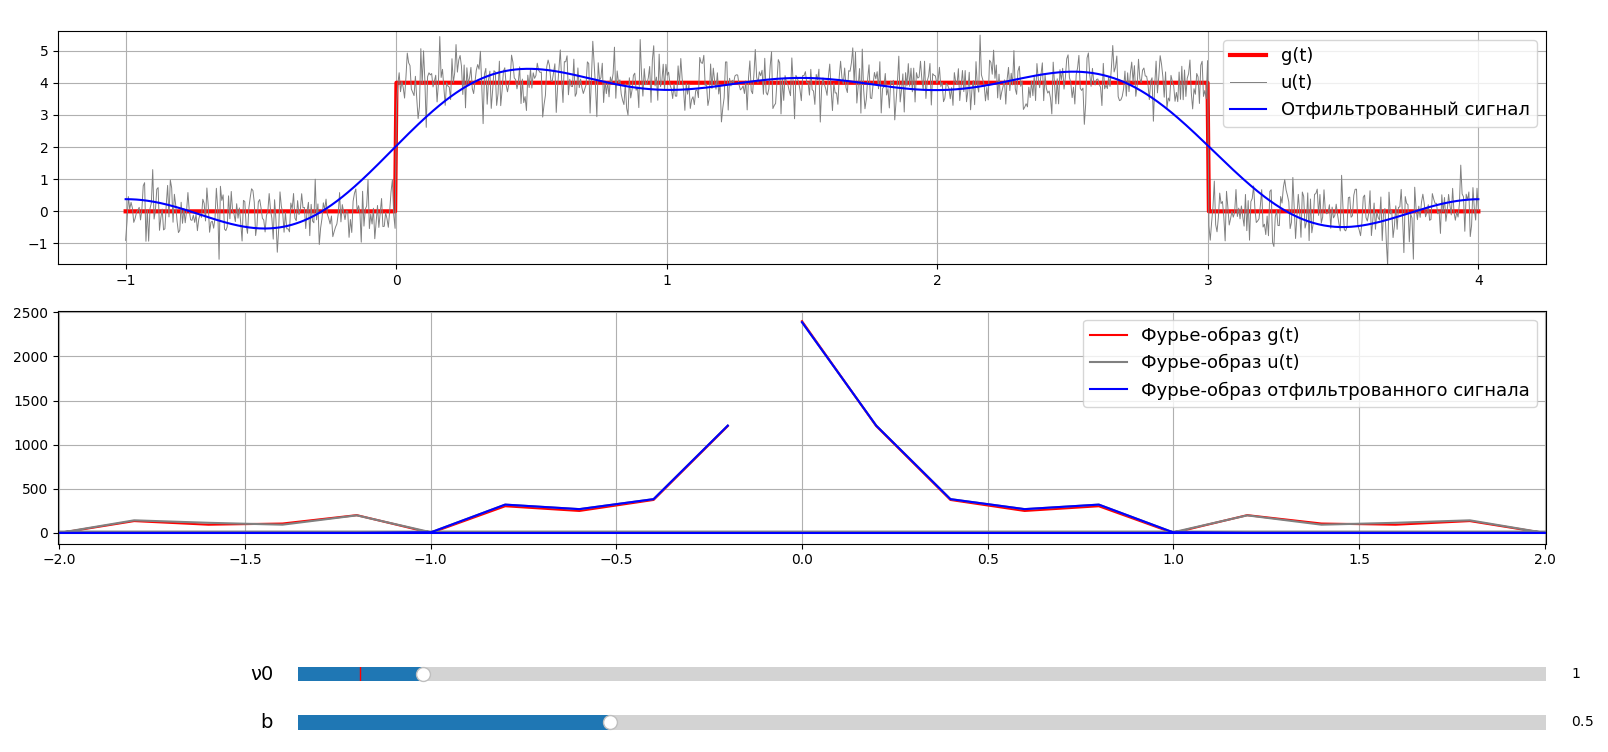
\includegraphics[width=1\textwidth]{../images/1.1_0.5_1.png}
    \caption{Графики при \(\nu_0 = 1\) и \(b = 0.5\)}  
    \label{fig:my_image}  
\end{figure}

\begin{figure}[H]  
    \centering
    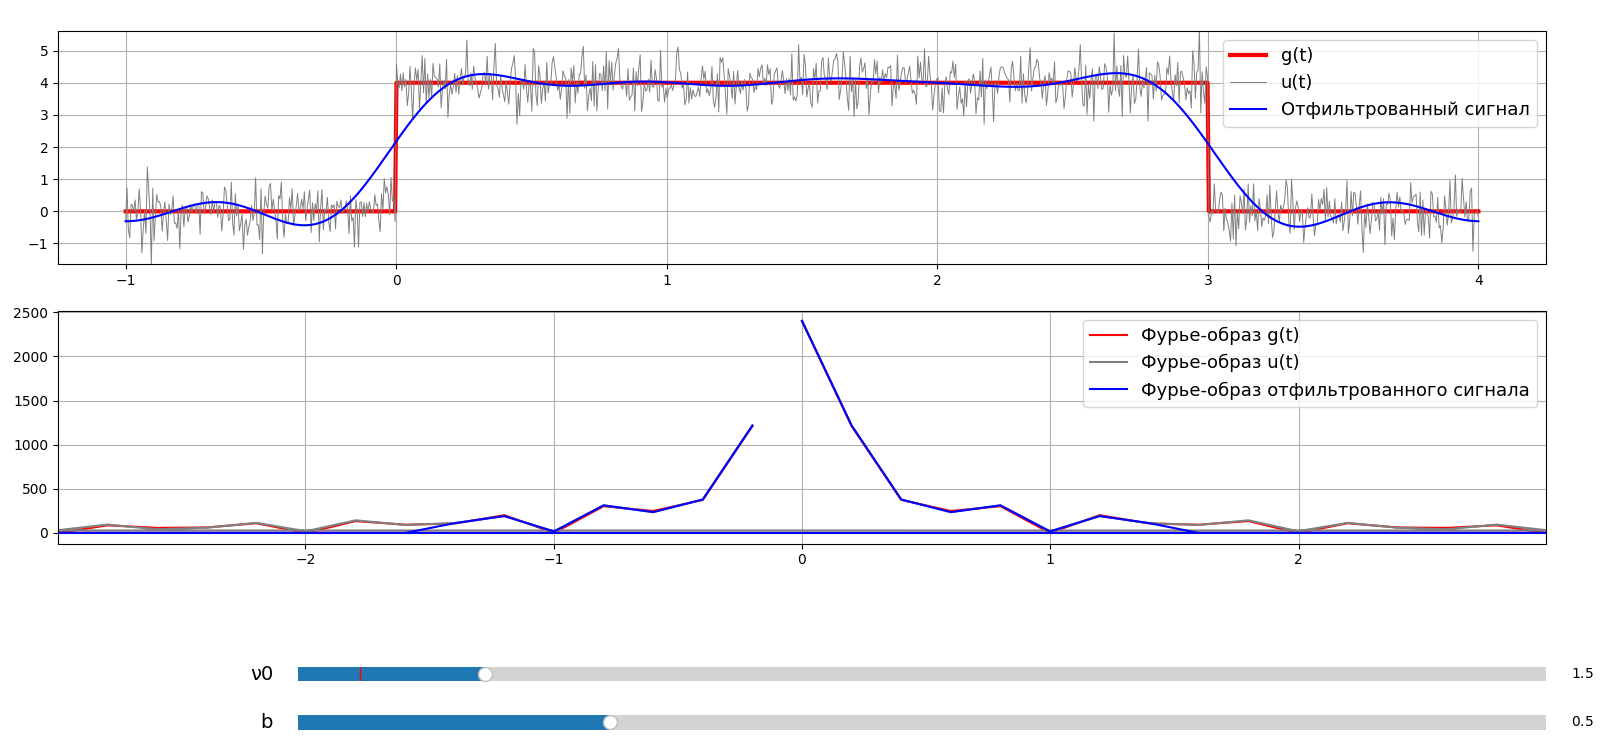
\includegraphics[width=1\textwidth]{../images/1.1_0.5_1.5.png}
    \caption{Графики при \(\nu_0 = 1.5\) и \(b = 0.5\)}  
    \label{fig:my_image}  
\end{figure}

\begin{figure}[H]  
    \centering
    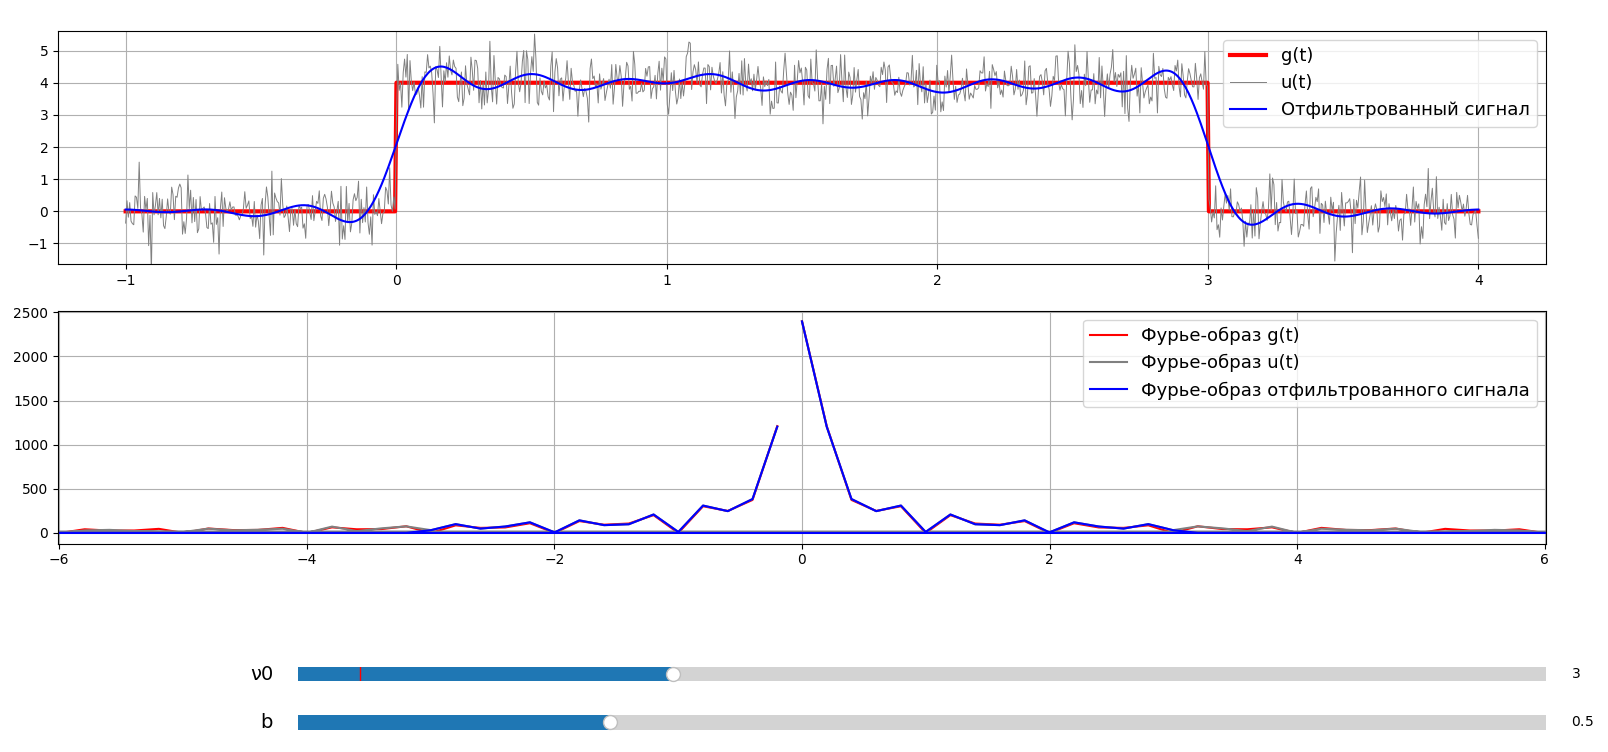
\includegraphics[width=1\textwidth]{../images/1.1_0.5_3.png}
    \caption{Графики при \(\nu_0 = 3\) и \(b = 0.5\)}  
    \label{fig:my_image}  
\end{figure}

\begin{figure}[H]  
    \centering
    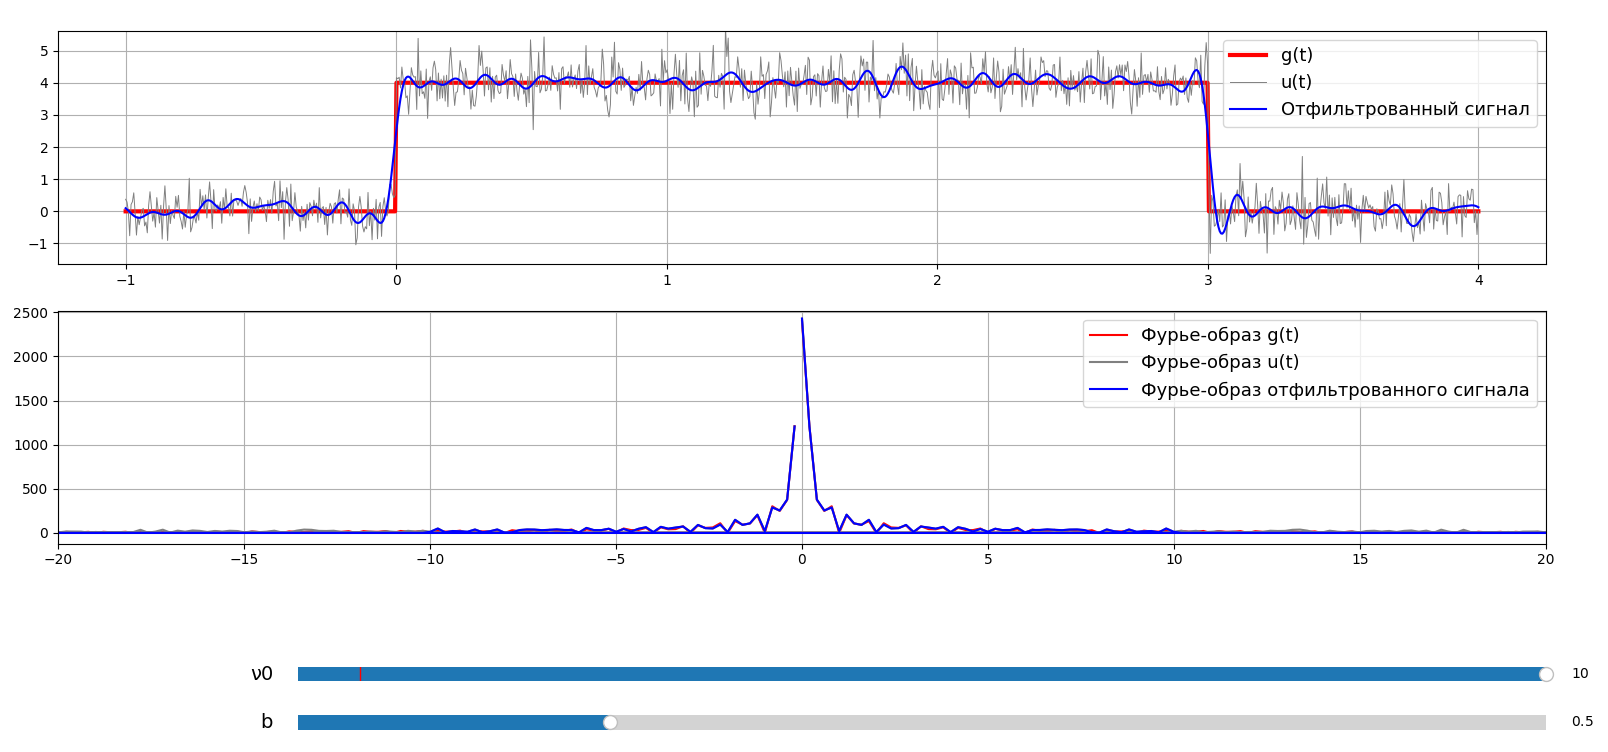
\includegraphics[width=1\textwidth]{../images/1.1_0.5_10.png}
    \caption{Графики при \(\nu_0 = 10\) и \(b = 0.5\)}  
    \label{fig:my_image}  
\end{figure}

\subsubsection{Вывод}

\begin{itemize}
    \item С увеличением \(\nu_0\) изменялось количество колебаний отфильтрованного сигнала. 
    Число гармоник увеличивалось, однако при большем значении \(\nu_0\) не всегда удавалось получить
    хорошо отфильтрованный сигнал. Наиболее удачным оказался график при параметрах \(\nu_0 = 3\) и \(b = 0.5\). 
    На этом графике форма отфильтрованного сигнала практически идеально совпадает с исходной, 
    а шум удалён наиболее эффективно.

    \item Можно заметить, что графики модулей Фурье-образов отфильтрованного сигнала и шума совпадают 
    при всех выбранных значениях \(\nu_0\). Теперь обратим внимание на синюю линию — модуль Фурье-образа. 
    С увеличением \(\nu_0\) синий график постепенно начинает совпадать с остальными, практически 
    полностью повторяя их форму. Это означает, что при увеличении частоты среза \(\nu_0\) фильтр 
    пропускает больше частот, что приводит к лучшему сохранению формы сигнала.


\end{itemize}

\subsubsection{Фиксирую \(\nu_0\)}

Для этого задания выберу несколько значений \(b = \set{0, 0.5, 1, 2}\),
чтобы исследовать поведение графиков при фиксированном значении \(\nu_0\ = 3\).
Это значение было выбрано, поскольку ранее мне показалось, что при этом значении
сигнал хорошо фильтруется.
Ниже рассмотрим эти графики:

\begin{figure}[H]  
    \centering
    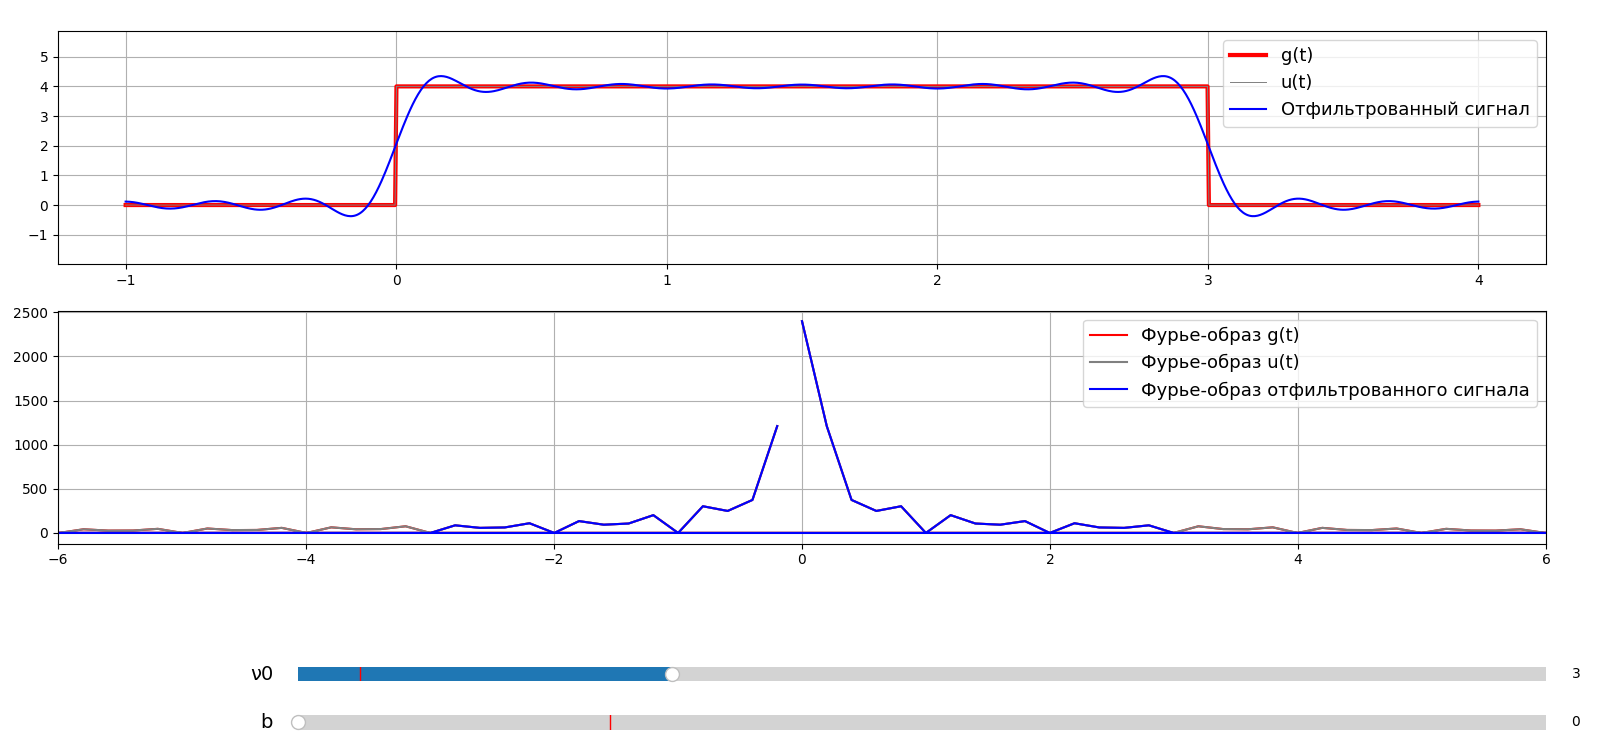
\includegraphics[width=1\textwidth]{../images/1.1_0_3.png}
    \caption{Графики при \(\nu_0 = 3\) и \(b = 0\)}  
    \label{fig:my_image}  
\end{figure}

\begin{figure}[H]  
    \centering
    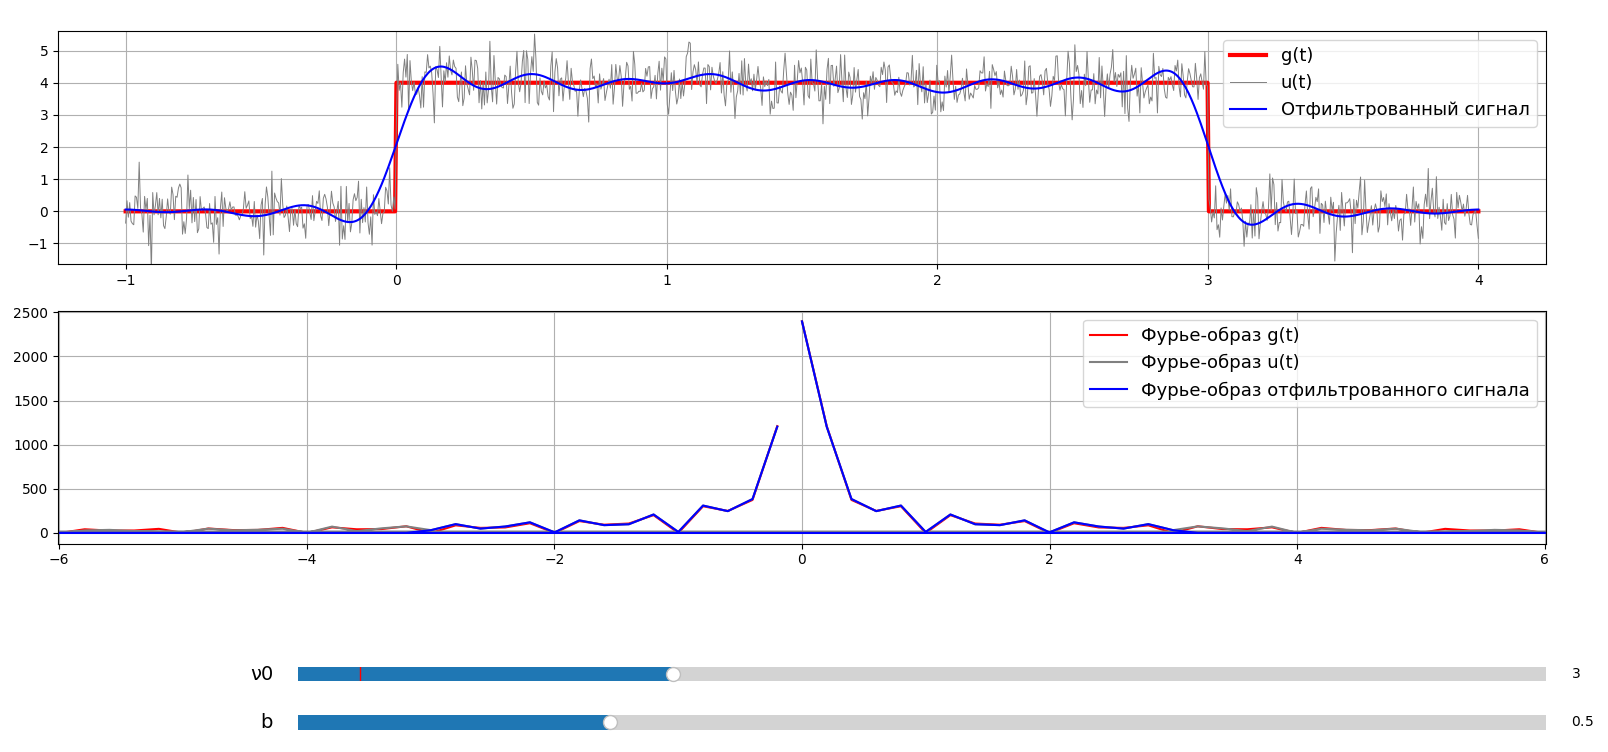
\includegraphics[width=1\textwidth]{../images/1.1_0.5_3.png}
    \caption{Графики при \(\nu_0 = 3\) и \(b = 0.5\)}  
    \label{fig:my_image}  
\end{figure}

\begin{figure}[H]  
    \centering
    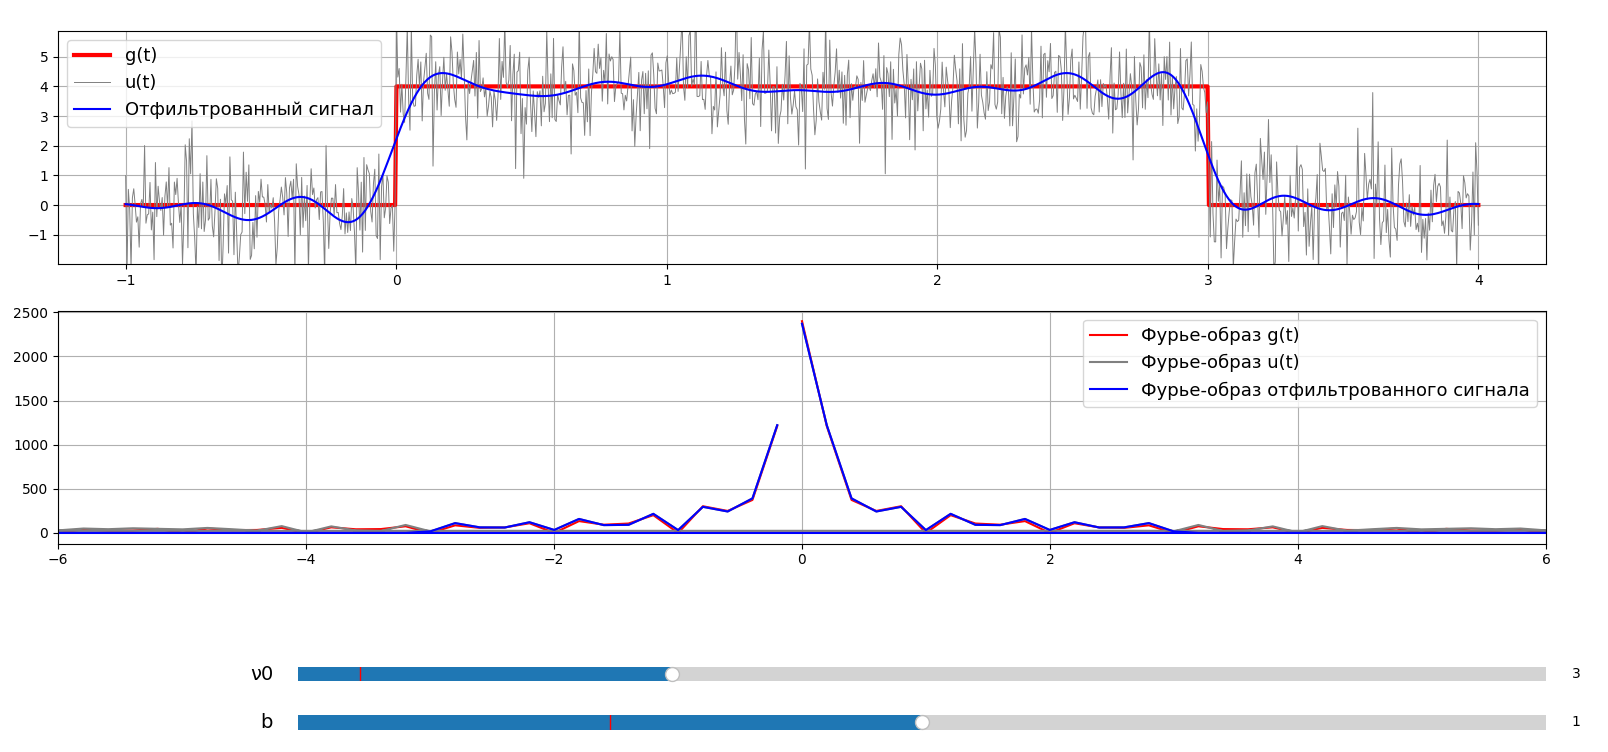
\includegraphics[width=1\textwidth]{../images/1.1_1_3.png}
    \caption{Графики при \(\nu_0 = 3\) и \(b = 1\)}  
    \label{fig:my_image}  
\end{figure}

\begin{figure}[H]  
    \centering
    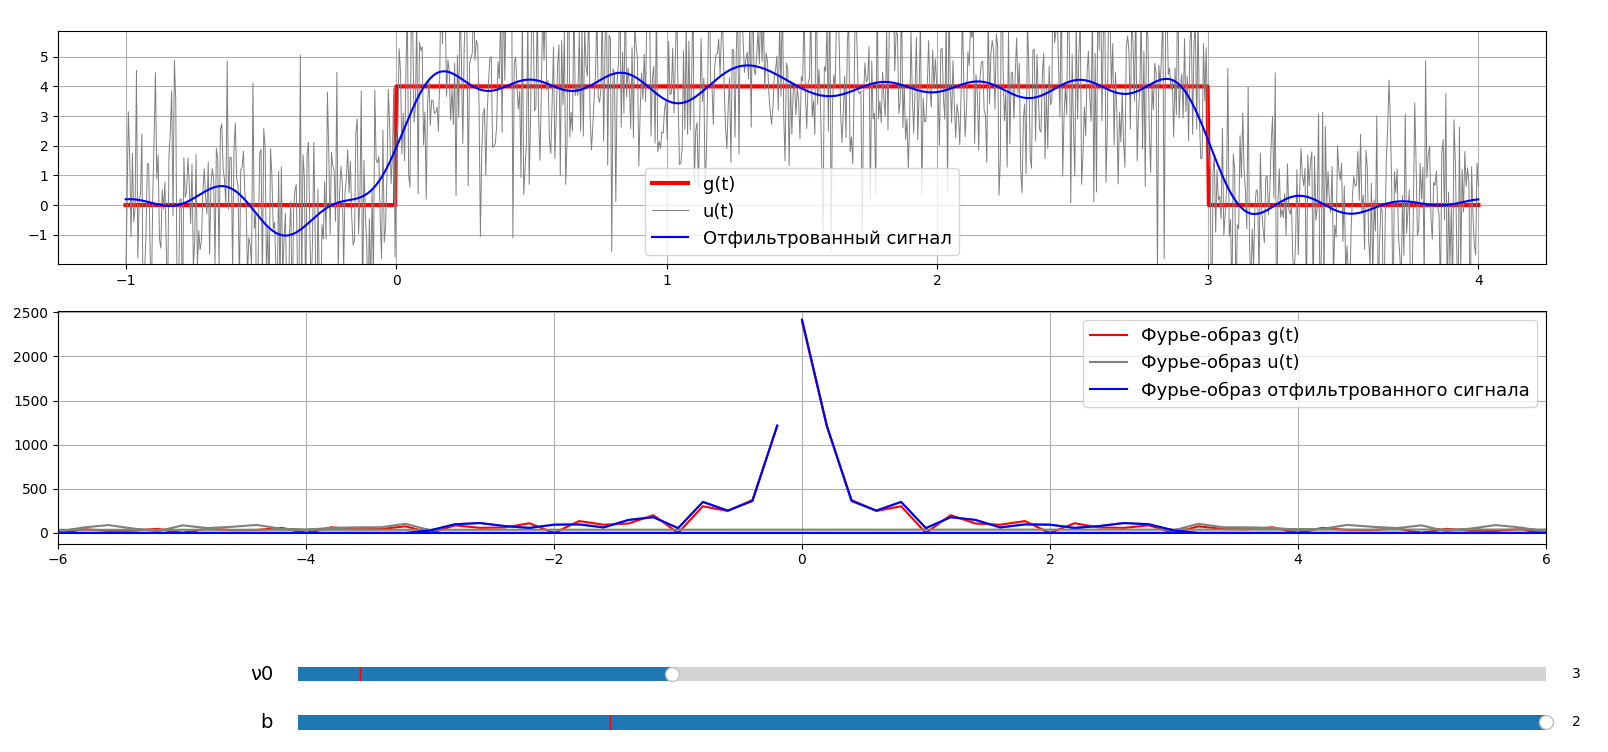
\includegraphics[width=1\textwidth]{../images/1.1_2_3.png}
    \caption{Графики при \(\nu_0 = 3\) и \(b = 2\)}  
    \label{fig:my_image}  
\end{figure}

\subsubsection{Вывод}

\begin{itemize}
    \item При увеличении \(b\) увеличивается шум, а также растет амплитуда колебаний
    синего графика. То есть чем больше шум, тем больше помех в отфильтрованном сигнале
    . Идеальным графиком будет первый, поскольку шума совсем нет, 
    соответственно мы фактически фильтруем не зашумленный сигнал, а идеальный.

    \item Спектр отфильтрованного сигнала близок к спектру \(g(t)\), но остаются небольшие шумовые компоненты.
    Различия между модулями фурье-образов слабо заметны при моих параметрах \(b\).

\end{itemize}





\subsection{Убираем специфические частоты}

\subsubsection{Предподготовка}

Для этого задания выберу параметры функций:
\[
a = 4, t_0 = 0, t_1 = 3, c = 1, d = 2, b = 0.5
\]

Значение частоты я выберу \(\nu_0 = 0.5\). Стоит указать, что это только начальные значения
и в ходе этого задания я буду их менять, чтобы посмотреть, как это отображается на 
графике.

У меня получатся следующие функции:

\[
g(t) = 
\begin{cases} 
4, & t \in [0, 3], \\
0, & t \notin [0, 3],
\end{cases}
\]

\[
u(t) = g(t) + 0.5\xi(t) + \sin(2t),
\]
где \(\xi(t) \sim U[-1, 1]\) — равномерное распределение на интервале \([-1, 1]\).

Отрисую график для выбранных значений:

\begin{figure}[H]  
    \centering
    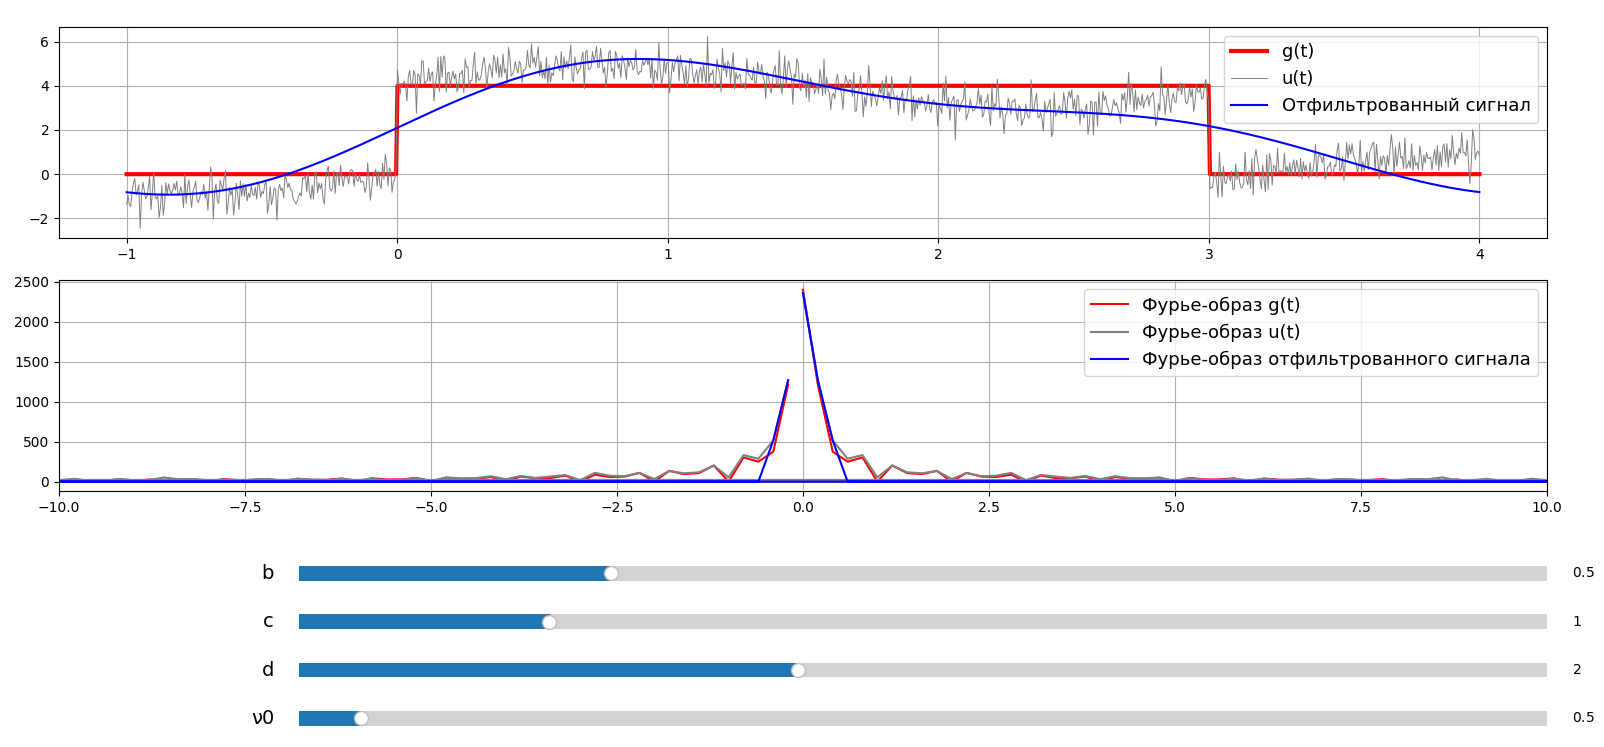
\includegraphics[width=1\textwidth]{../images/1.2.png}
    \caption{Графики при \(b = 0.5\), \(c =  1\), \(d = 1\) и \(\nu_0 = 3\)}  
    \label{fig:my_image}  
\end{figure}

В отличие от предыдущего пункта можно заметить, что шум пошел по синусоиде.

В этом задании нужно сделать совмещенный фильтр - он убирает не только низкие
частоты, но и гармонические колебания. Алгоритм задания такой же, как и описыватся в \
пункте \hyperlink{mytext}{1.1.1}.

Также отмечу, что, поскольку нужно исследовать довольно много меняющихся параметров
в этом задании, я приведу несколько показательных случаев в следующих пунктах
 и отражу влияние компонент в выводе.

\subsubsection{Случай, когда \(b = 0\)}

Отдельно рассмотрю случай, когда \(b = 0\). Вот несколько графиков


\begin{figure}[H]  
    \centering
    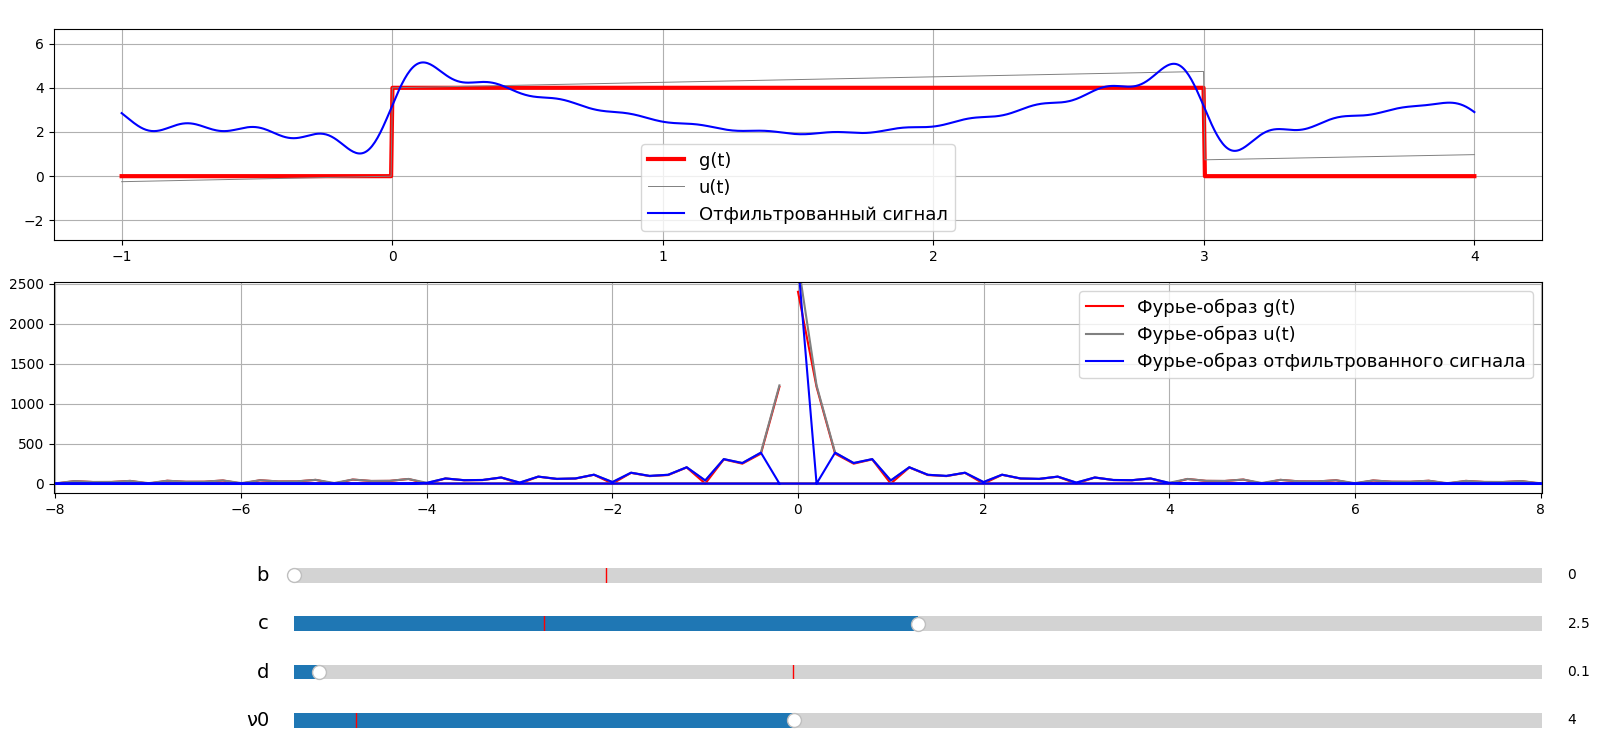
\includegraphics[width=1\textwidth]{../images/1.2.1.png}
    \caption{Графики при \(b = 0\), \(c =  2.5\), \(d = 0.1\) и \(\nu_0 = 4\)}  
    \label{fig:my_image}  
\end{figure}


\begin{figure}[H]  
    \centering
    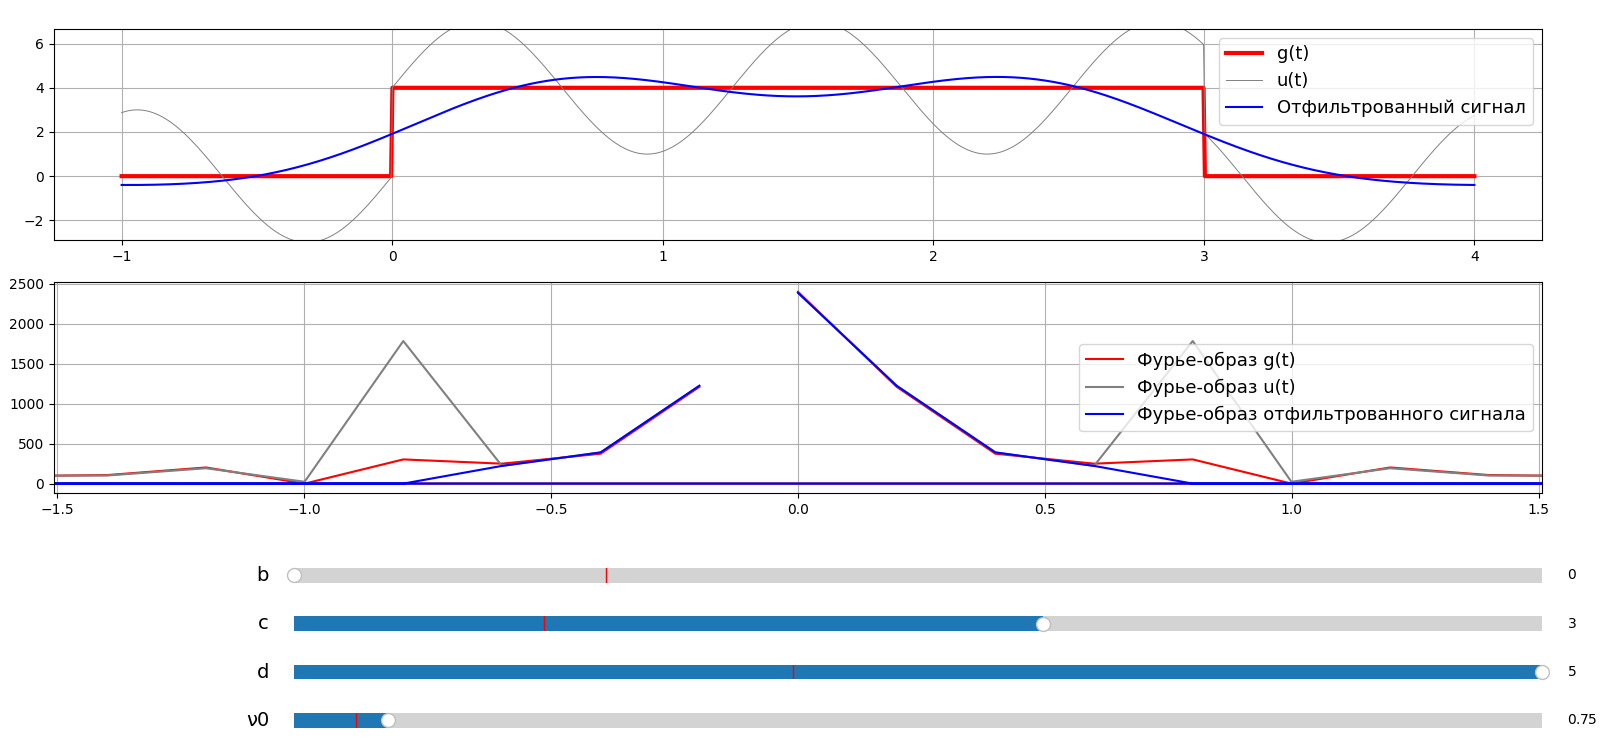
\includegraphics[width=1\textwidth]{../images/1.2.2.png}
    \caption{Графики при \(b = 0\), \(c =  3\), \(d = 5\) и \(\nu_0 = 0.75\)}  
    \label{fig:my_image}  
\end{figure}


\begin{figure}[H]  
    \centering
    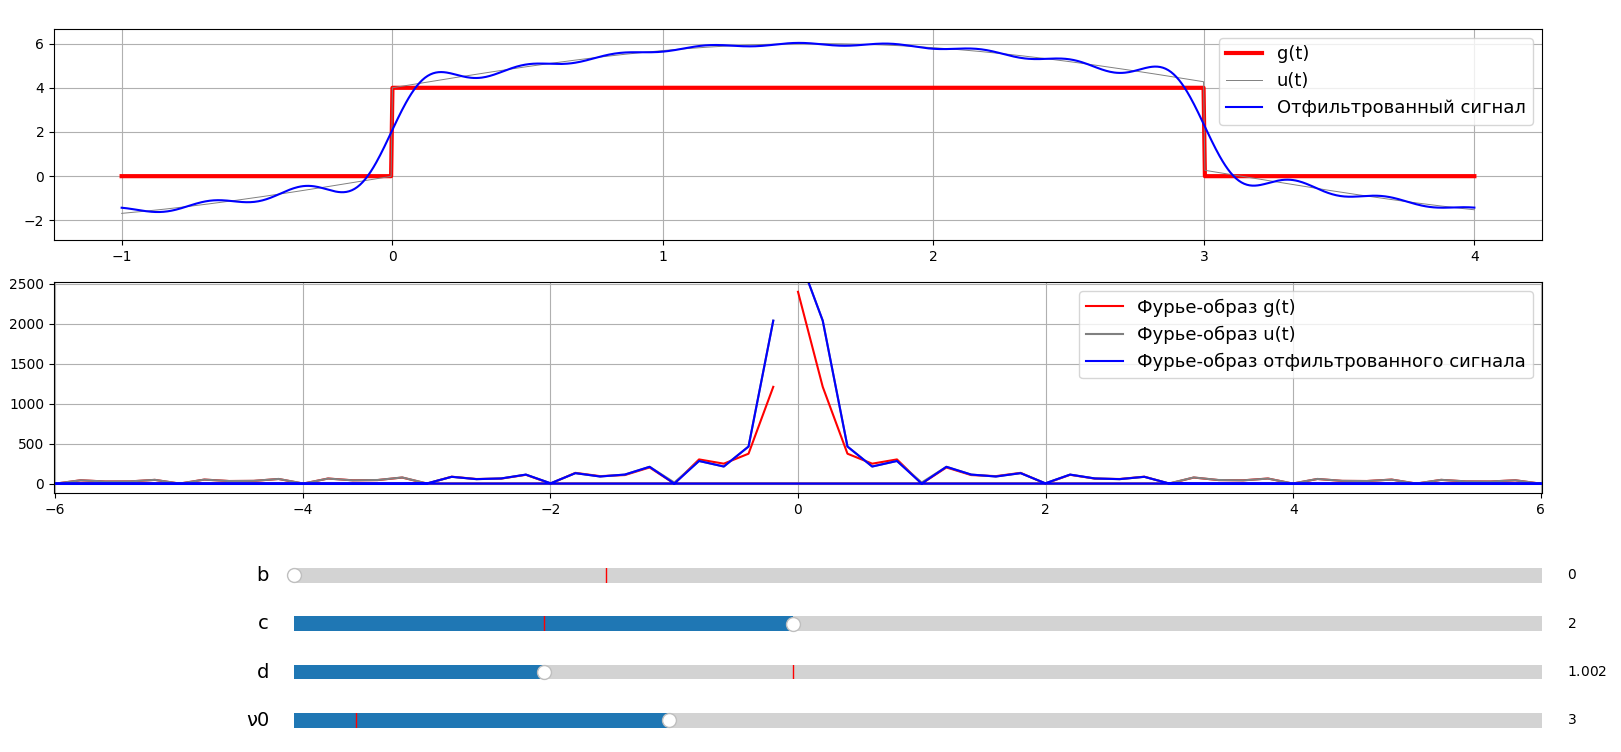
\includegraphics[width=1\textwidth]{../images/1.2.3.png}
    \caption{Графики при \(b = 0\), \(c =  2\), \(d \approx 1\) и \(\nu_0 = 3\)}  
    \label{fig:my_image}  
\end{figure}

\subsubsection{Остальные случаи}

Приведу графики, когда \(b \neq 0\):

\begin{figure}[H]  
    \centering
    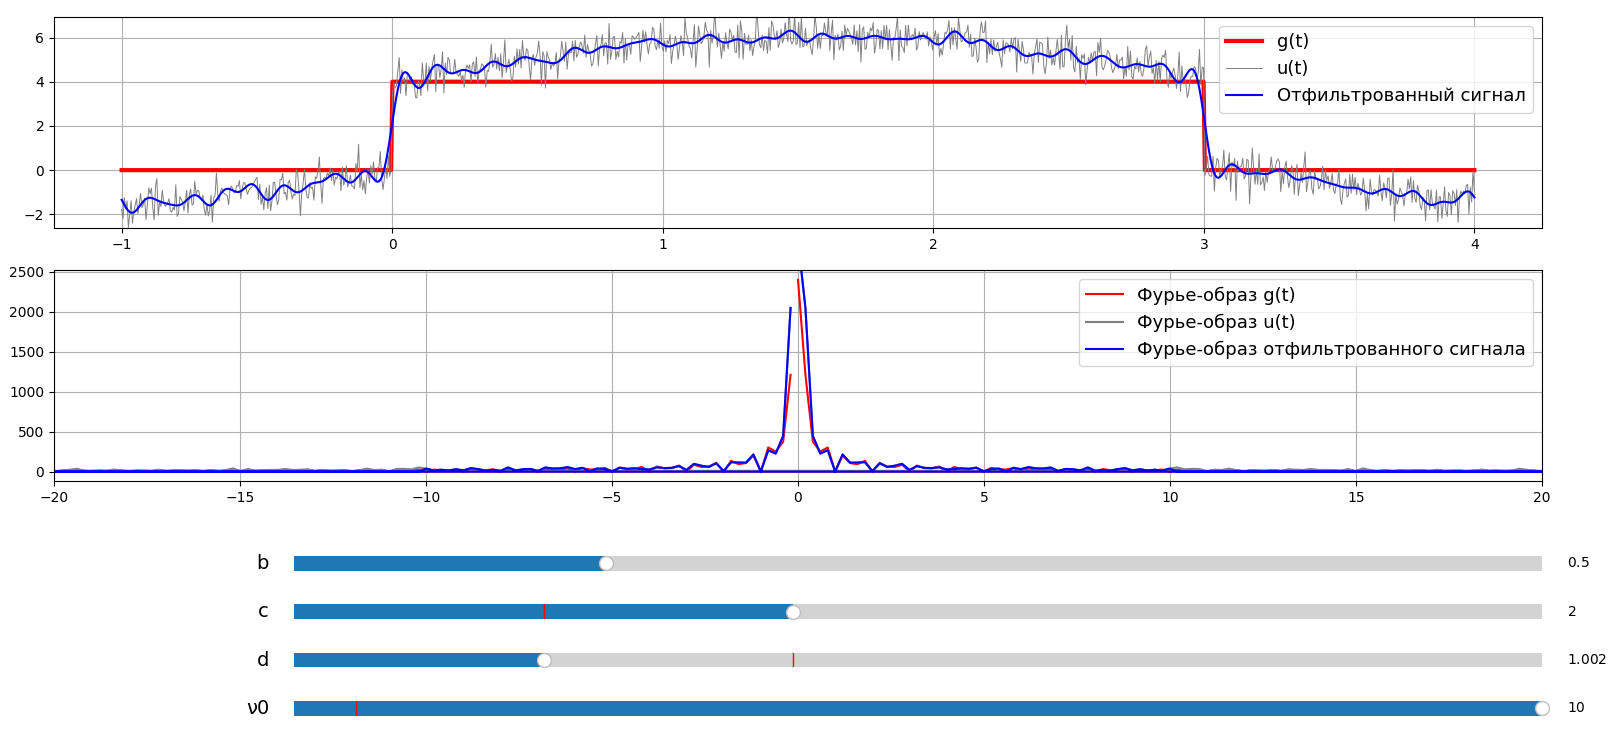
\includegraphics[width=1\textwidth]{../images/1.3.1.png}
    \caption{Графики при \(b = 2\), \(c =  0.75\), \(d \approx 5\) и \(\nu_0 = 1\)}  
    \label{fig:my_image}  
\end{figure}


\begin{figure}[H]  
    \centering
    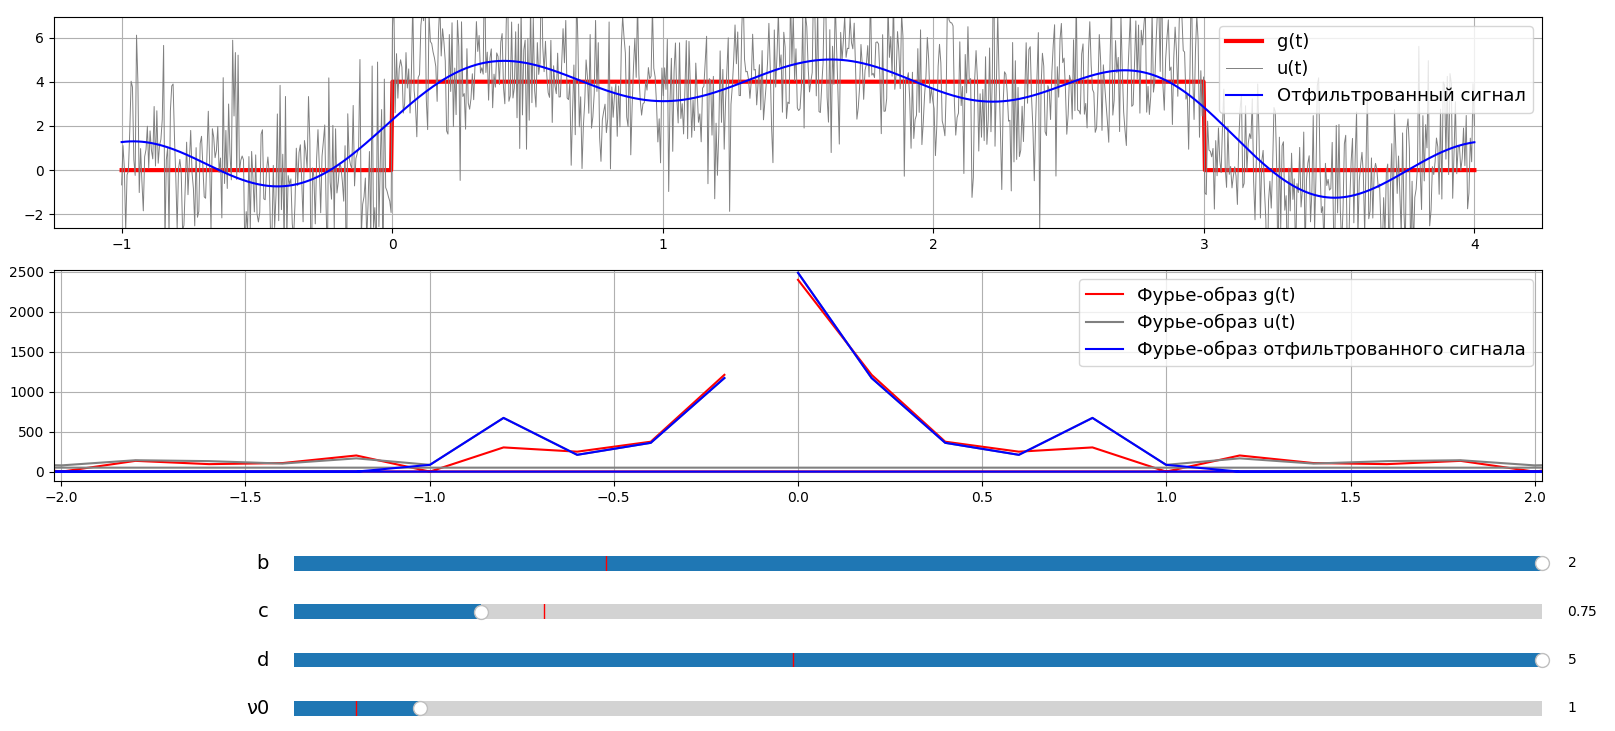
\includegraphics[width=1\textwidth]{../images/1.3.2.png}
    \caption{Графики при \(b = 0\), \(c =  3\), \(d = 5\) и \(\nu_0 = 0.75\)}  
    \label{fig:my_image}  
\end{figure}


\begin{figure}[H]  
    \centering
    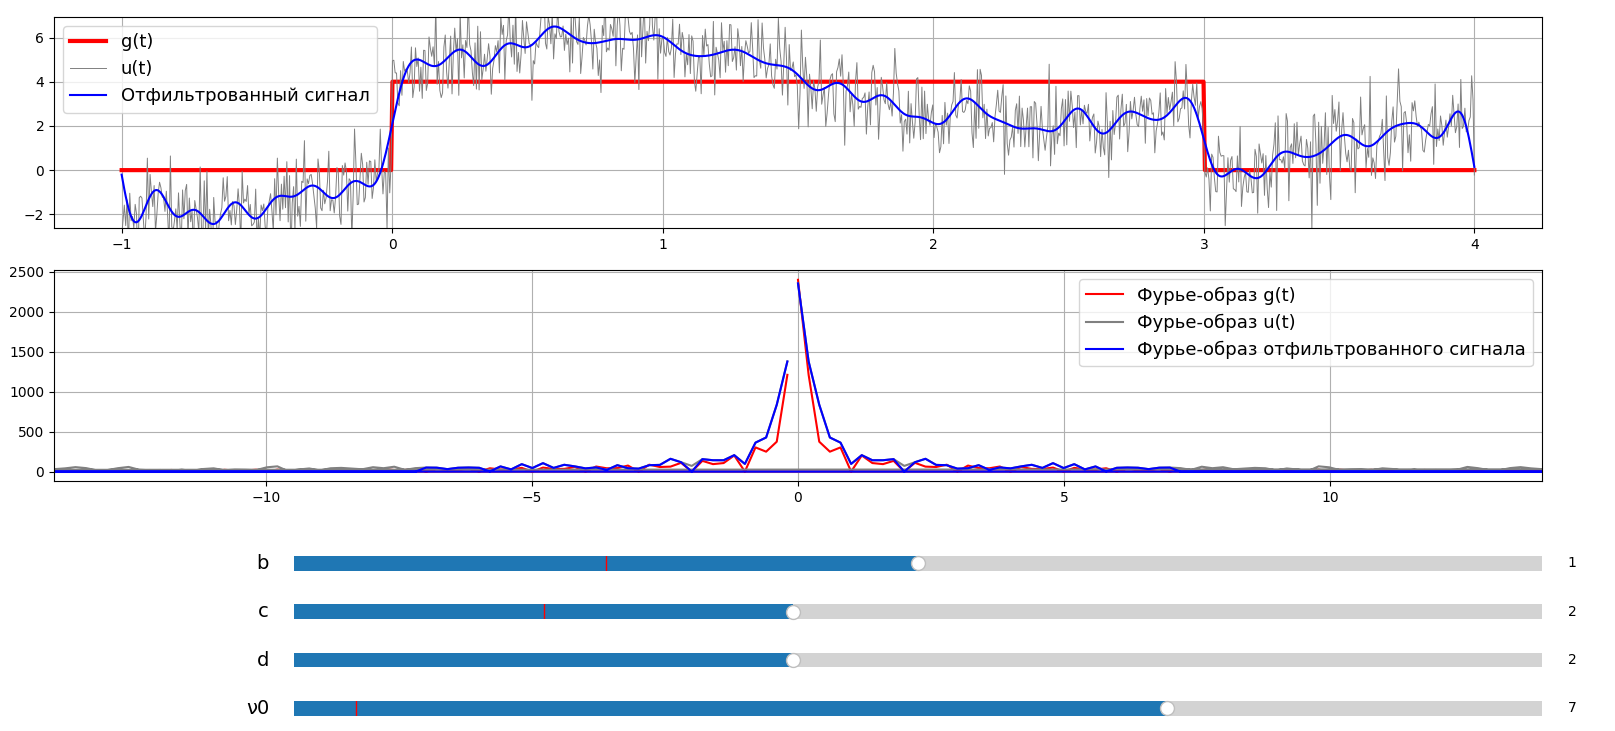
\includegraphics[width=1\textwidth]{../images/1.3.3.png}
    \caption{Графики при \(b = 1\), \(c =  2\), \(d = 2\) и \(\nu_0 = 7\)}  
    \label{fig:my_image}  
\end{figure}


\subsubsection{Выводы по пунктам 1.3.2 и 1.3.3}

Много раз поменяв параметры \(b\), \(c\), \(d\) и \(\nu_0\), я пришла к следующим выводам:
\begin{itemize}
    \item Параметр \(b\): Чем больше значение \(b\), тем больше шума накладывается на сигнал. Это связано с тем, что \(b\) определяет амплитуду шума.
    \item Параметр \(c\): Увеличение \(c\) приводит к увеличению амплитуды колебаний зашумлённой функции. Также \(c\) влияет на количество колебаний шума, делая их более частыми или редкими.
    \item Параметр \(d\): Увеличение \(d\) приводит к увеличению частоты гармонической составляющей шума, что делает колебания более частыми.
    \item Параметр \(\nu_0\): Чем больше частота среза \(\nu_0\), тем больше колебаний сохраняется в отфильтрованном сигнале. Это связано с тем, что фильтр пропускает больше высокочастотных компонент.
\end{itemize}

На графиках заметно, что совмещенный фильтр эффективно работает при присутствии
колебаний в зашумленной функциии.

\subsection{Убираем низкие частоты?}
\subsubsection{Предподготовка}
Для начала в этом задании я выберу такие функции:
\[
g(t) = 
\begin{cases} 
4, & t \in [0, 3], \\
0, & t \notin [0, 3],
\end{cases}
\]

\[
u(t) = g(t) + 0.5\xi(t) + \sin(2t),
\]
где \(\xi(t) \sim U[-1, 1]\) — равномерное распределение на интервале \([-1, 1]\).

И пропущу функцию \(u(t)\) через фильтр, который обнуляет фурье-образ в 
окресности точки \(v = 0\)

\subsubsection{Графики}

Изображу график для выбранных ранее параметров:

\begin{figure}[H]  
    \centering
    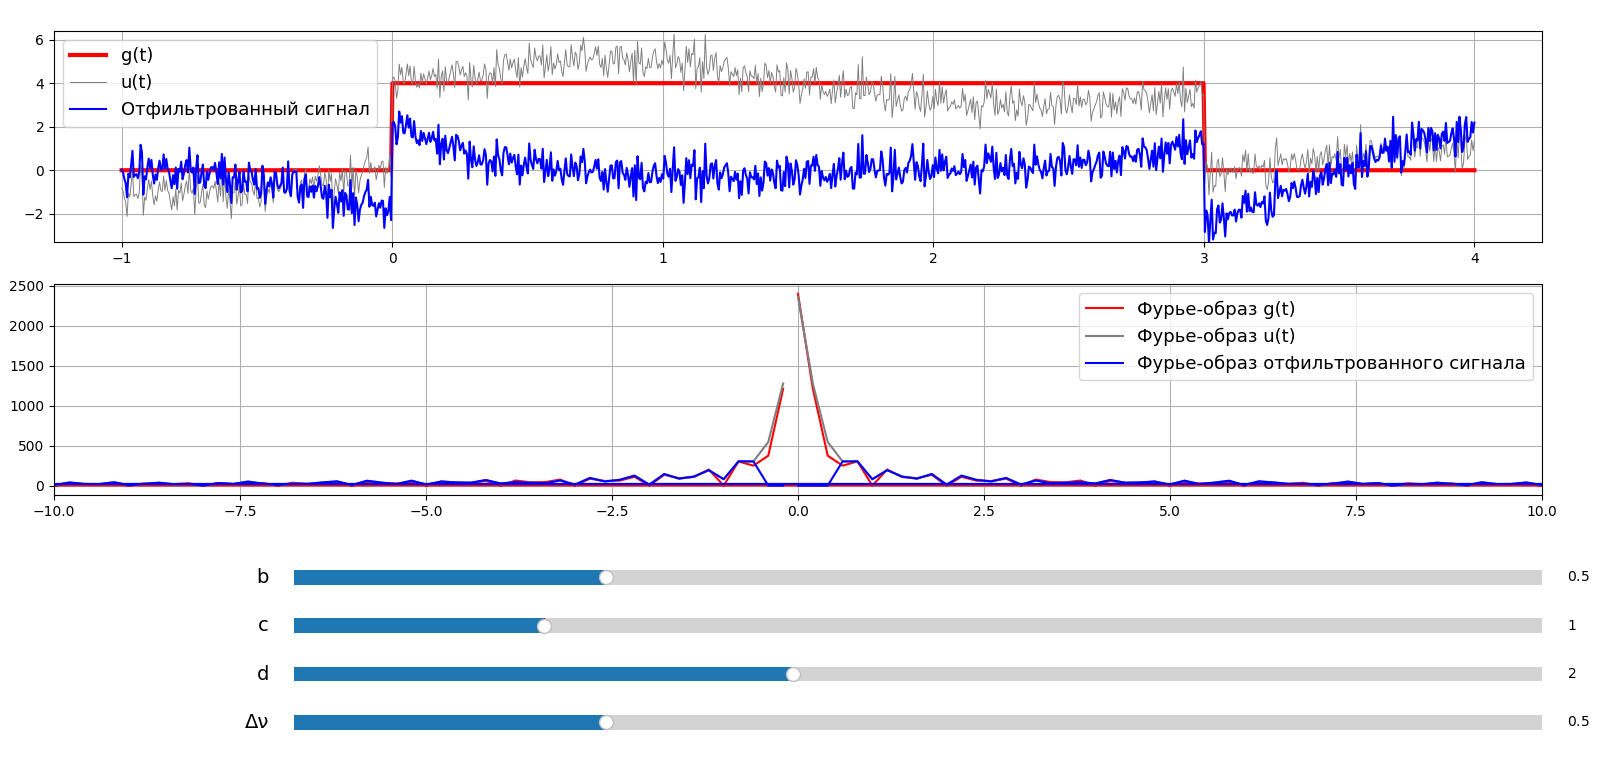
\includegraphics[width=1\textwidth]{../images/1.4.1.png}
    \caption{Графики при \(b = 0.5\), \(c =  1\), \(d = 2\) и \(\varDelta  v = 0.5\)}  
    \label{fig:my_image}  
\end{figure}

Далее буду менять окрестность точки \(v\) - \(\varDelta v = \set{0, 1}\) для
трех наборов параметров \(b\), \(c\), \(d\), которые будут отражены внизу рисунка.


\begin{figure}[H]  
    \centering
    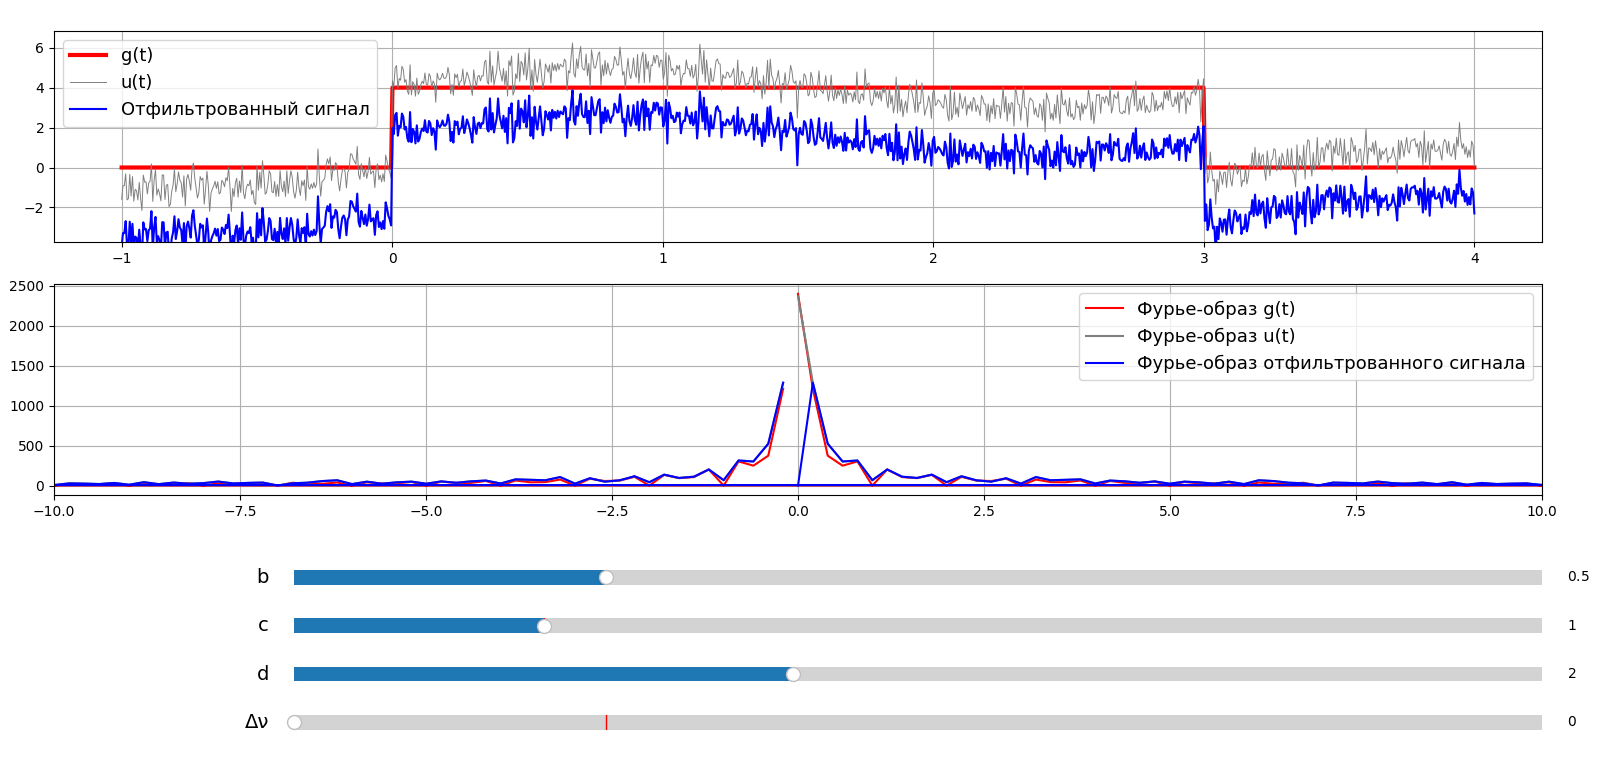
\includegraphics[width=1\textwidth]{../images/1.4.2.png}
    \caption{Графики при \(b = 0.5\), \(c =  1\), \(d = 2\) и \(\varDelta  v = 0\)}  
    \label{fig:my_image}  
\end{figure}


\begin{figure}[H]  
    \centering
    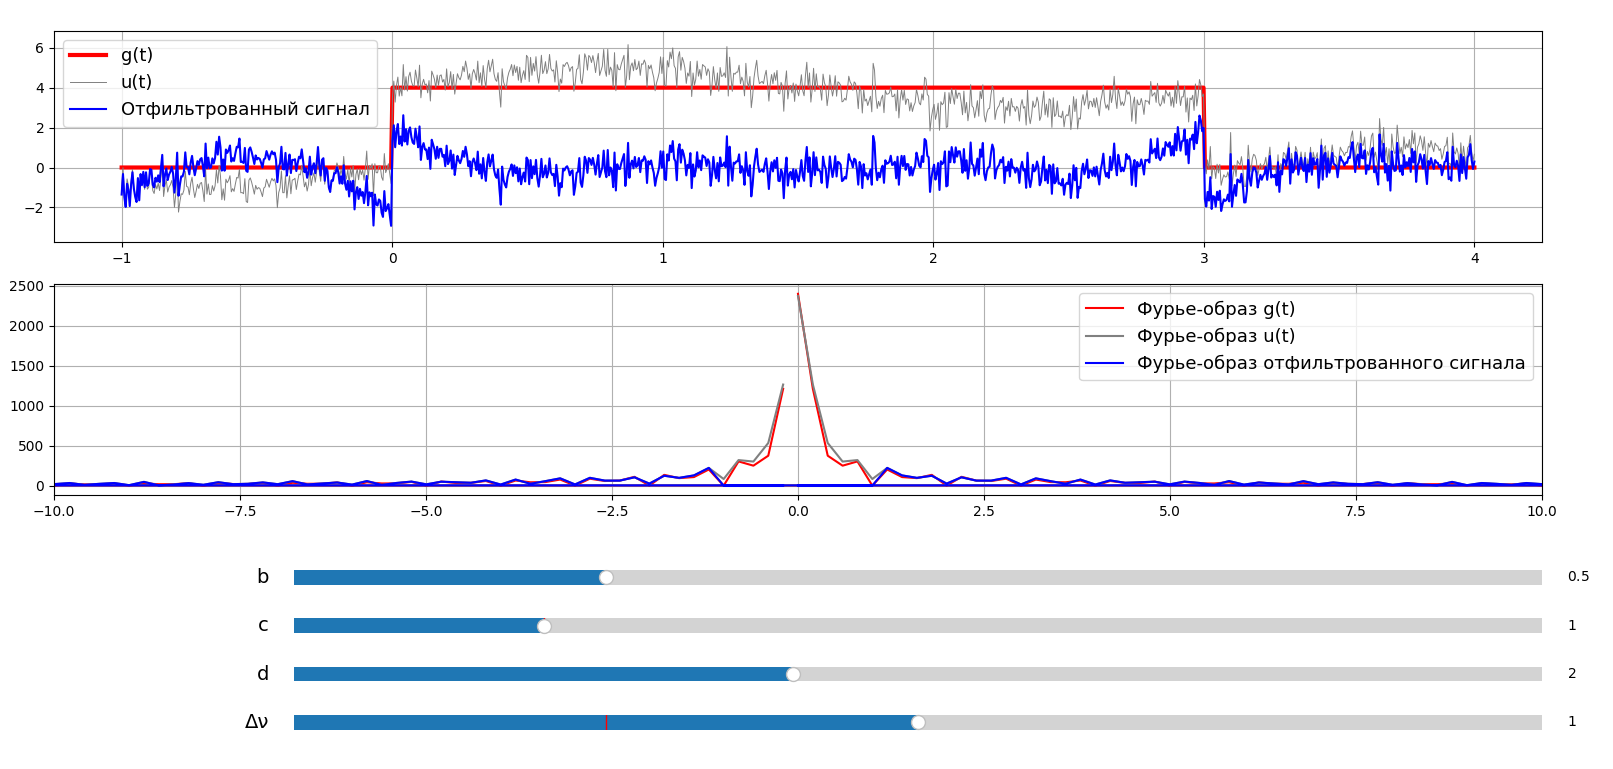
\includegraphics[width=1\textwidth]{../images/1.4.3.png}
    \caption{Графики при \(b = 0.5\), \(c =  1\), \(d = 2\) и \(\varDelta  v = 1\)}  
    \label{fig:my_image}  
\end{figure}


\begin{figure}[H]  
    \centering
    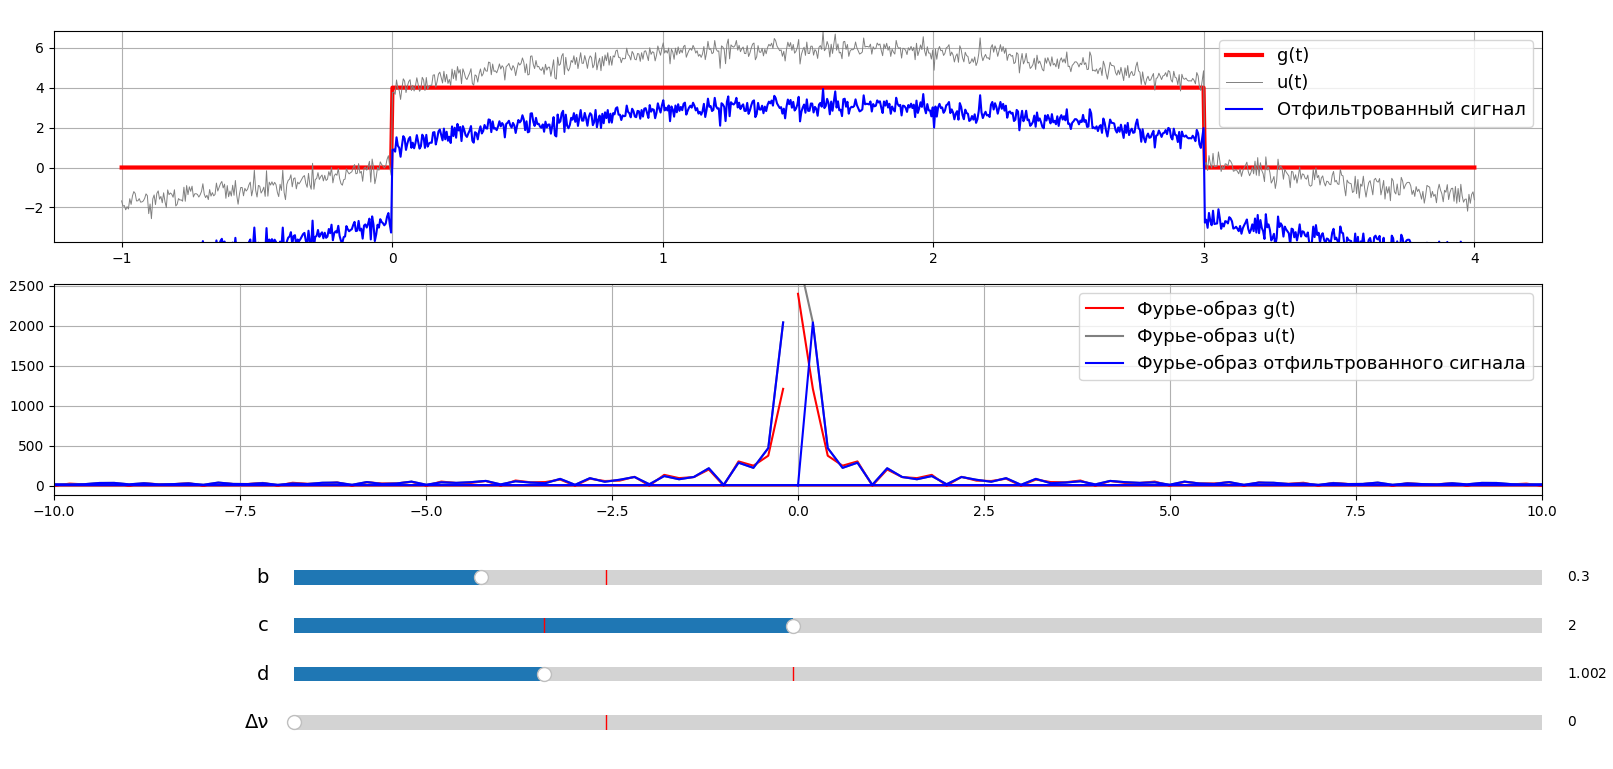
\includegraphics[width=1\textwidth]{../images/1.4.4.png}
    \caption{Графики при \(b = 0.3\), \(c =  2\), \(d \approx 1\) и \(\varDelta  v = 0\)}  
    \label{fig:my_image}  
\end{figure}

\begin{figure}[H]  
    \centering
    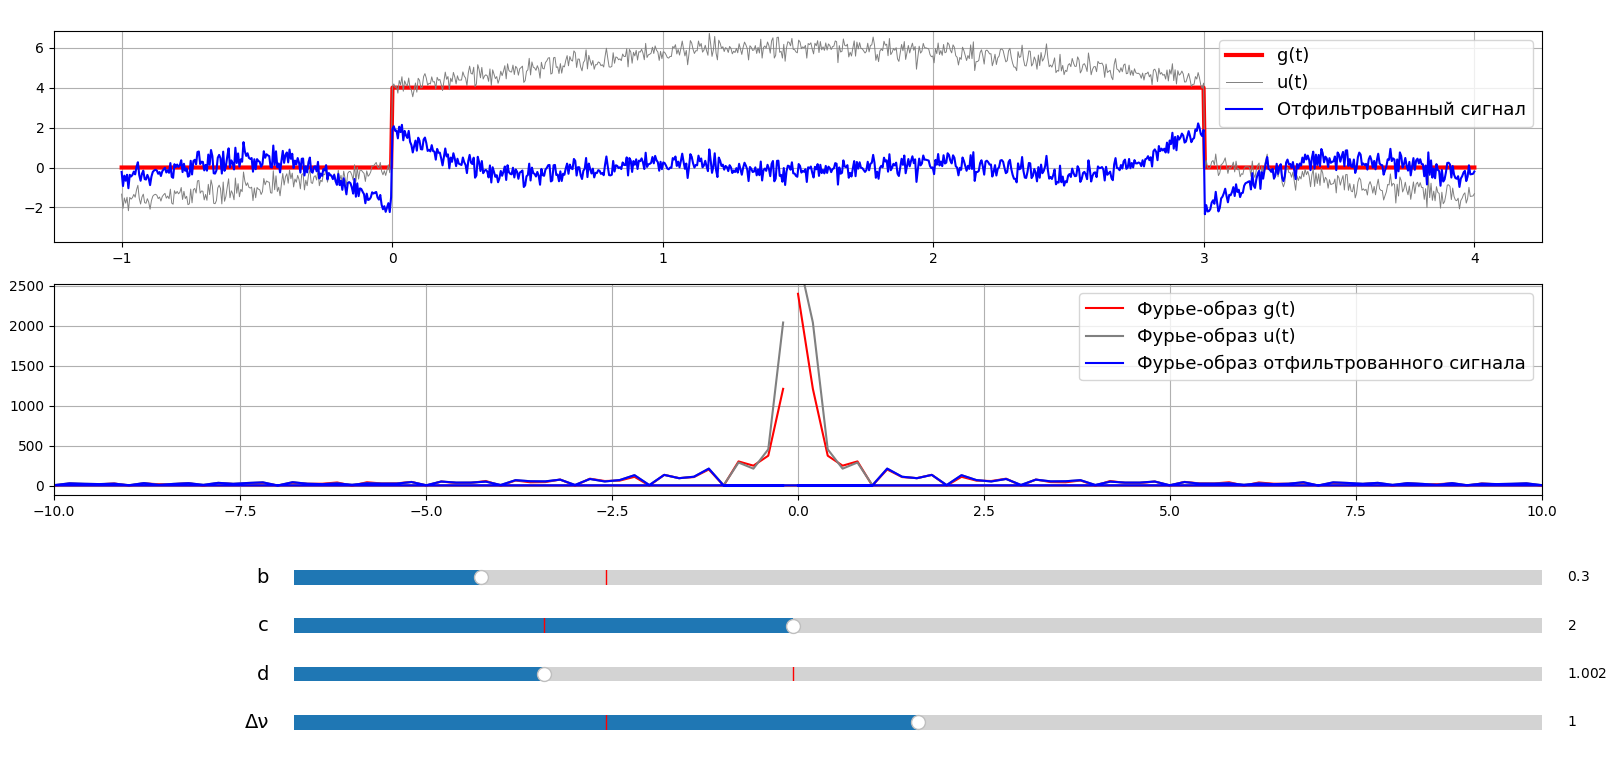
\includegraphics[width=1\textwidth]{../images/1.4.5.png}
    \caption{Графики при \(b = 0.3\), \(c =  2\), \(d \approx 1\) и \(\varDelta  v = 1\)}  
    \label{fig:my_image}  
\end{figure}


\begin{figure}[H]  
    \centering
    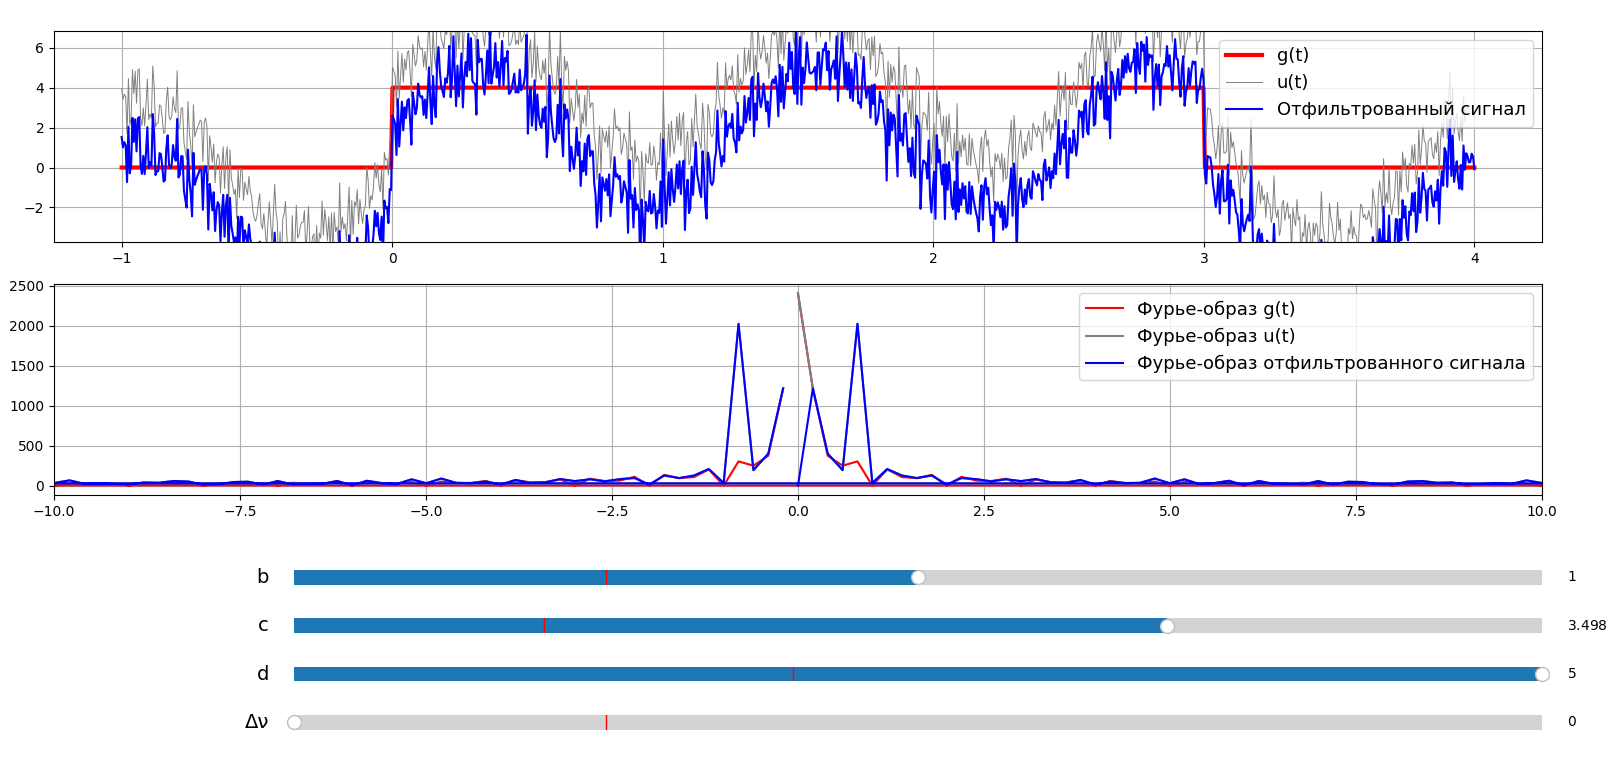
\includegraphics[width=1\textwidth]{../images/1.4.6.png}
    \caption{Графики при \(b = 1\), \(c \approx 3.5\), \(d = 5\) и \(\varDelta  v = 0\)}  
    \label{fig:my_image}  
\end{figure}


\begin{figure}[H]  
    \centering
    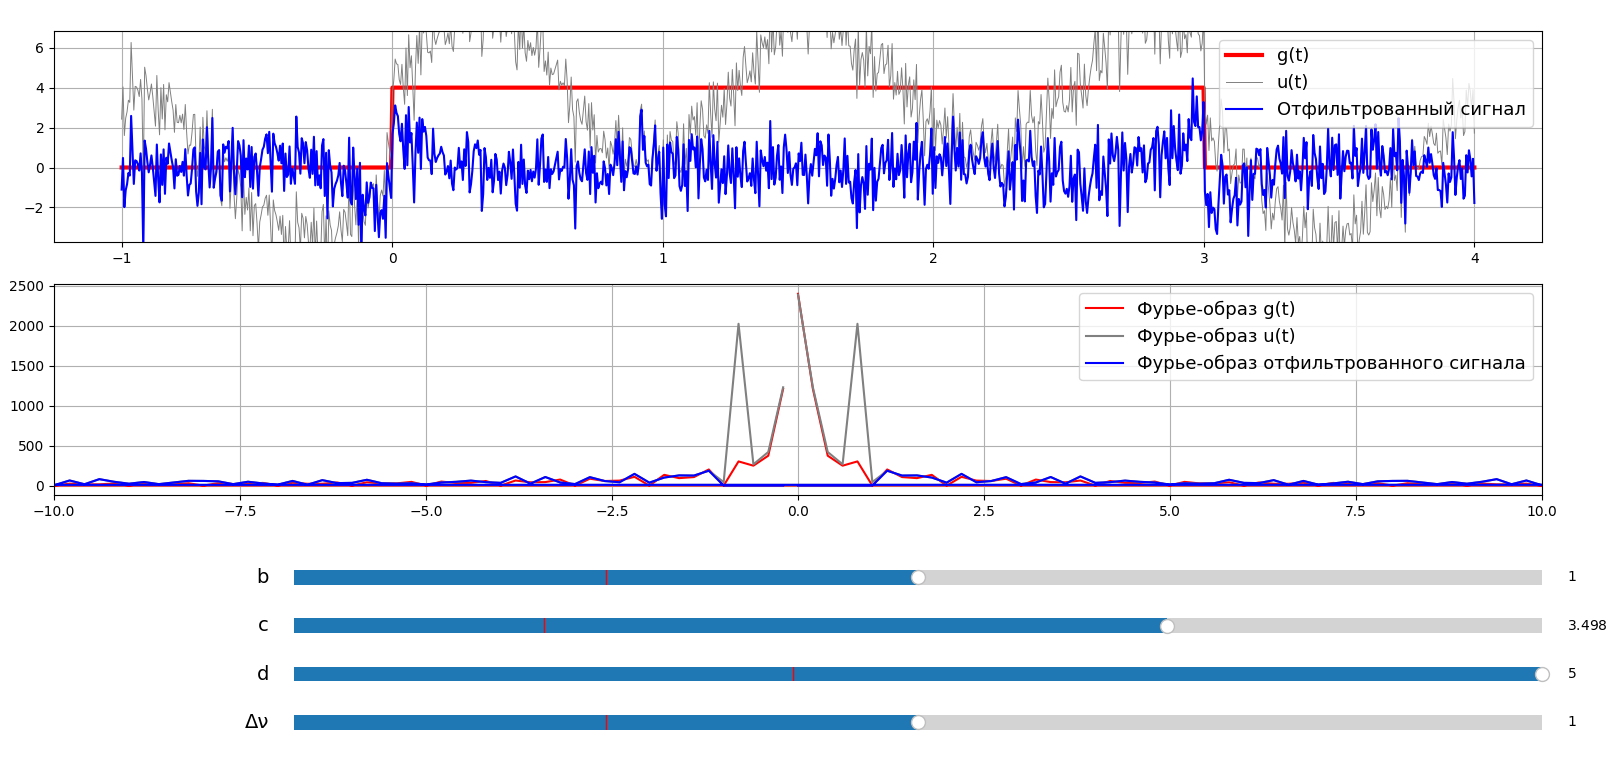
\includegraphics[width=1\textwidth]{../images/1.4.7.png}
    \caption{Графики при \(b = 1\), \(c \approx 3.5\), \(d = 5\) и \(\varDelta  v = 1\)}  
    \label{fig:my_image}  
\end{figure}


\subsubsection{Выводы}

\begin{itemize}
    \item На графиках видно, что при разных значениях частот среза изменяется степень фильтрации и форма сигнала.
    \item Фильтр успешно подавляет низкочастотные компоненты сигнала, что видно по изменению формы отфильтрованного сигнала и его Фурье-образа. Низкочастотные компоненты вблизи \(\nu\) практически отсутствуют после фильтрации.
    \item Однако данный фильтр не является идеальным решением. Подавление низких частот в сигнале может быть не всегда целесообразным, так как низкочастотные компоненты часто содержат полезную информацию. Кроме того, шум в высокочастотной области сигнала сохраняется, что может ухудшить качество обработки.
\end{itemize}
Таким образом, проведенный анализ подтверждает, что фильтр низких частот эффективно справляется с задачей подавления низкочастотных компонент сигнала, но его использование может быть ограничено из-за сохранения шума и возможного искажения полезной информации.

\section{Task. Фильтрация звука}
\subsection{Краткое условие}

\end{document}
